\documentclass{article}

\textwidth=6.5in
\textheight=8.5in
\voffset=-54pt
\oddsidemargin=0in
\evensidemargin=0in
\setlength{\parskip}{8pt}
\setlength{\parindent}{0pt}

\usepackage{workbook}

\usepackage[]{handout}

\begin{document}

\begin{center}
  \large\textsc{Problem Set 25 - The Fundamental Theorem of Calculus, Part 2}
  
      \pspace{12pt}
  \begin{problemonly}\large Name: \rule{5cm}{0.15mm}\\ \end{problemonly}
\end{center}

\begin{enumerate}
\item For help with these problems, you may wish to read the worked examples on pp. 761-771 in Gottlieb.

  \begin{enumerate}
  \item \label{gottlieb-24.1.5}

    \begin{problem}
      Find the area under the graph of $y=e^x$ between $x=0$ and $x=1$.
    \end{problem}

    \pspace{\vfill}

    \begin{solution} % Jason Bland
      This area is $\displaystyle \int_0^1 e^x \, dx = e^x \Big|_0^1 =
      \boxed{e - 1}$.
    \end{solution}

  \item \label{gottlieb-24.1.6a}

    \begin{problem}
      Find the area under the graph of $y=e^{-x}$ between $x=-1$ and
      $x=0$.
    \end{problem}

    \pspace{\vfill}

    \begin{solution} % Jason Bland
      This area is $\displaystyle \int_{-1}^0 e^{-x} \, dx = -e^{-x}
      \Big|_{-1}^0 = \boxed{e - 1}$.
    \end{solution}

  \item \label{gottlieb-24.1.6b}

    \begin{problem}
      Find the area under the graph of $y=e^{-x}$ between $x=0$ and $x=1$.
    \end{problem}

    \pspace{\vfill}

    \begin{solution} % Jason Bland
      This area is $\displaystyle \int_0^1 e^{-x} \, dx = -e^{-x}
      \Big|_0^1 = \boxed{1 - e^{-1}}$.
    \end{solution}

  \item
    \begin{problem}
      Sketch the areas described in \ref{gottlieb-24.1.5},
      \ref{gottlieb-24.1.6a}, and \ref{gottlieb-24.1.6b}.  Does the
      relative size of your answers make sense with your sketches?  (By
      ``relative size'', we mean: do your pictures and calculations agree
      on which of the areas is biggest / smallest?)
    \end{problem}

    \pspace{\stretch{2}}

    \begin{solution} 
      Here are the three areas:      
      \begin{center}
        \begin{tabular}{ccccc}
          \begin{tikzpicture}
            \begin{axis}[width=2in, xtick={-1, 1}, ytick={1}]
              \addplot+[domain=-1.1:1.1, black] {e^x} node[left]{$y = e^x$};
              \addplot+[domain=0:1, plusarea] {e^x} \closedcycle;
            \end{axis}
          \end{tikzpicture} & \hspace{0.2in} & 
          \begin{tikzpicture}
            \begin{axis}[width=2in, xtick={-1, 1}, ytick={1}]
              \addplot+[domain=-1.1:1.1, black] {e^(-x)} node[pos=0,
              right]{$y = e^{-x}$};
              \addplot+[domain=-1:0, plusarea] {e^(-x)} \closedcycle;
            \end{axis}
          \end{tikzpicture} & \hspace{0.2in} & 
          \begin{tikzpicture}
            \begin{axis}[width=2in, xtick={-1, 1}, ytick={1}]
              \addplot+[domain=-1.1:1.1, black] {e^(-x)} node[pos=0,
              right]{$y = e^{-x}$};
              \addplot+[domain=0:1, plusarea] {e^(-x)} \closedcycle;
            \end{axis}
          \end{tikzpicture} \\
          \ref{gottlieb-24.1.5} && \ref{gottlieb-24.1.6a} &&
          \ref{gottlieb-24.1.6b} 
        \end{tabular}        
      \end{center}
      The region in \ref{gottlieb-24.1.6a} is  the region in
      \ref{gottlieb-24.1.5} reflected over the $y$-axis, so they have the
      same area.  The region in \ref{gottlieb-24.1.6b} is 
      smaller.  This agrees with the answers we calculated. 
    \end{solution}

  \end{enumerate}

  \pspace{\newpage}

\item
  Suppose the temperature of an object is changing at a rate of $r(t) =
  -2e^{-t}$ degrees Celsius per hour, where $t$ is given in hours.

  \begin{enumerate}

  \item
    \begin{problem}
      Is the object heating or cooling?
    \end{problem}
    \pspace{\vfill}

    \begin{solution}
      $r(t)$ is always negative, so the object is \fbox{cooling}. 
    \end{solution}

  \item
    \begin{problem}
      Between time $t=0$ and $t=1$, how much does the temperature change?
    \end{problem}
    \pspace{\vfill}

    \begin{solution}
      The temperature changes by $\displaystyle \int_0^1 r(t)\,dt$.  One
      antiderivative of $r(t) = - 2 e^{-t}$ is $2 e^{-t}$, so
      $\displaystyle \int_0^1 r(t)\,dt = 2 e^{-t} \Big|_0^1 =
      \boxed{\frac{2}{e} - 2}$. 
    \end{solution}

  \item
    \begin{problem}
      Between $t=1$ and $t=2$, how much does the temperature change?
    \end{problem}
    \pspace{\vfill}

    \begin{solution}
      The temperature changes by $\displaystyle \int_1^2 r(t)\,dt = 2
      e^{-t} \Big|_1^2 = \boxed{\frac{2}{e^2} - \frac{2}{e}}$. 
    \end{solution}

  \item
    \begin{problem}
      If the object was 100 degrees Celsius at time $t=0$, how hot is it
      at time $t=1$?
    \end{problem}
    \pspace{\vfill}

    \begin{solution}
      The temperature at $t = 1$ is $100 + \displaystyle \int_0^1 r(t)\,dt
      = 100 + \left( \frac{2}{e} - 2 \right) = \boxed{98 + \frac{2}{e}}$.
    \end{solution}

  \end{enumerate}

  \pspace{\newpage}

\item \label{norovirus-rate}

  In February 2025, several people on campus got norovirus.  Suppose $r(t)
  = 6 - 3 \sqrt{t}$ models the rate of change of the number of people on
  campus with norovirus in people per day, where $t$ is measured in days
  and $t = 0$ represents February 10.  On February 14, 100 people on
  campus had norovirus.
  \begin{enumerate}
  \item
    \begin{problem}
      Based on the model, how many people on campus had norovirus on February 19?
    \end{problem}
    \pspace{\vfill}

    \begin{solution}
      The number of people with norovirus on February 19 was
      $\displaystyle 100+\int_4^9(6-3\sqrt{t})\,dt$.  One antiderivative
      of $6 - 3 \sqrt{t} = 6 - 3 t^{1/2}$ is $6t - 2 t^{3/2}$, so
      \begin{align*}
        100 + \int_4^9(6-3\sqrt{t})\,dt &= 100 + \Big[ 6t -
          2 t^{3/2} \Big]_4^9 \\
        &= 100 + \left( \left[ 54 - 2 \cdot 27 \right] - \left[ 24
            - 2 \cdot 8 \right] \right) \\
        &= \boxed{92}
      \end{align*}
    \end{solution}

  \item
    \begin{problem}
      Based on the model, how many people on campus had norovirus on February 11?
    \end{problem}
    \pspace{\vfill}

    \begin{solution}
      The number of people with norovirus on February 11 was
      \begin{align*}
        100 + \int_4^1(6-3\sqrt{t})\,dt &= 100 + \Big[ 6t -
          2 t^{3/2} \Big]_4^1 \\
        &= 100 + \left( \left[ 6 - 2 \cdot 1 \right] - \left[ 24
            - 2 \cdot 8 \right] \right) \\
        &= \boxed{96}
      \end{align*}
    \end{solution}

  \item
    \begin{problem}
      At what times between February 10 and February 20 was the number of
      people with norovirus increasing?  At what times was it decreasing?
    \end{problem}
    \pspace{\stretch{2}}

    \begin{solution}
      We can answer this by figuring out when $r(t) = 6 - 3 \sqrt{t}$ is
      positive or negative; that is, we want to make a sign chart for
      $r(t)$.  So, we should first figure out when $r(t)$ is 0:
      \begin{align*}
        6 - 3 \sqrt{t} &= 0 \\
        6 &= 3 \sqrt{t} \\
        2 &= \sqrt{t} \\
        4 &= t
      \end{align*}
      Then, we can test a value less than 4 and a value greater than 4;
      for example, $r(1) = 6 - 3 > 0$ and $r(9) = 6 - 3 \cdot 3 < 0$.
      That gives us the following sign chart for $r(t)$:
      \begin{center}
        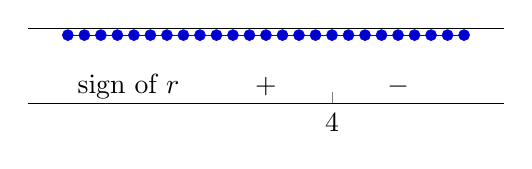
\begin{tikzpicture}
          \begin{axis}[axis y line=none, x axis line style={-}, xtick={4.}, xticklabels={$4$}, ymin=-2, height=1in, width=3in]
            \addplot+[domain=3.8:4.1, very thin]{0};
            \draw (axis cs: 3.8, -1.5) node[right] {sign of $r$};
            \draw (axis cs: 3.95, -1.5) node{$+$};
            \draw (axis cs: 4.05, -1.5) node{$-$};
          \end{axis}
        \end{tikzpicture}        
      \end{center}
      So, the number of people is increasing until February 14 and
      decreasing after that. 
    \end{solution}

  \item
    \begin{problem}
      Are your answers consistent with each other and with the fact that
      100 people had norovirus on February 14?
    \end{problem}
    \pspace{\vfill}

    \begin{solution}
      Yes, February 14 was the peak, so the number of cases on February 11
      and 19 should both be lower than 100.
    \end{solution}

  \end{enumerate}

\pspace{\newpage}

\item \label{ftoc2-ln-Mb} 

  \begin{enumerate}
  \item
    \begin{problem}
      Evaluate $\displaystyle \int_1^5 \frac{1}{t}\,dt$.
    \end{problem}
    \pspace{\vfill}

    \begin{solution}
      One antiderivative of $\frac{1}{t}$ is $\ln t$, so 
      \begin{align*}
        \int_1^5 \frac{1}{t}\,dt &= \ln t \Big|_1^5 \\
        &= \ln 5 - \ln 1 \\
        &= \boxed{\ln 5}
      \end{align*}
    \end{solution}

  \item \label{ftoc2-ln-integrate-1}
    \begin{problem}
      Evaluate $\displaystyle \int_1^x \frac{1}{t}\,dt$.
    \end{problem}
    \pspace{\vfill}

    \begin{solution}
      \begin{align*}
        \int_1^x \frac{1}{t}\,dt &= \ln t \Big|_1^x \\
        &= \ln x - \ln 1 \\
        &= \boxed{\ln x}
      \end{align*}
    \end{solution}

  \item
    \begin{problem}
      Find a value of $x > 1$ such that the area under the graph $y =
      \frac{1}{t}$ from 1 to $x$ is exactly 1.
    \end{problem}
    \pspace{\vfill}

    \begin{solution}
      The area under the graph $y = \frac{1}{t}$ from $t = 1$ to $t = x$
      is $\displaystyle \int_1^x \frac{1}{t}\,dt$, which we found in
      \ref{ftoc2-ln-integrate-1} was just $\ln x$.  So, we're looking for
      a value of $x > 1$ such that $\ln x = 1$, and the only such value is
      $\boxed{x = e}$.
    \end{solution}

  \item
    \begin{problem}
      Sketch a graph of $\frac{1}{t}$, and use it to explain why your
      formula for \ref{ftoc2-ln-integrate-1} doesn't work for $x < 0$. 
    \end{problem}
    \pspace{\stretch{2}}

    \begin{solution}
      Here is the graph of $\frac{1}{t}$:
      \begin{center}
        \begin{tikzpicture}
          \begin{axis}[width=2.5in, height=2.5in, xmin=-5, xmax=5,
            ymin=-5, ymax=5, xtick=\empty, ytick=\empty]
            \addplot+[domain=-5:5] {1/x};
          \end{axis}
        \end{tikzpicture}
      \end{center}
      Since the graph has a vertical asymptote at $t = 0$, it's not clear
      how to integrate from $t = 1$ to a negative value of $t$.  (If you
      take Math 1b, you'll investigate this issue much more!)
    \end{solution}

  \item
    \begin{problem}
      Find $\displaystyle \int_{-5}^{-1} \frac{1}{t}\,dt$.  (Hint: Use
      your sketch, and take advantage of symmetry.)
    \end{problem}
    \pspace{\vfill}

    \begin{solution}
      From our sketch, we can see that $\displaystyle \int_{-5}^{-1}
      \frac{1}{t}\,dt$ (a negative signed area, shown in red below) is the
      negative of $\displaystyle \int_1^5 \frac{1}{t}\,dt$:
      \begin{center}
        \begin{tikzpicture}
          \begin{axis}[width=3in, height=3in, xmin=-6, xmax=6,
            ymin=-6, ymax=6, xtick={-5, -1, 1, 5}, ytick=\empty]
            \addplot+[domain=-5:-1, minusarea] {1/x} \closedcycle;
            \addplot+[domain=1:5, plusarea] {1/x} \closedcycle;
            \addplot+[domain=-6:6, black] {1/x};            
          \end{axis}
        \end{tikzpicture}
      \end{center}
      Since we already found that $\displaystyle \int_1^5 \frac{1}{t}\,dt
      = \ln 5$, we can conclude that $\displaystyle \int_{-5}^{-1}
      \frac{1}{t}\,dt = \boxed{-\ln 5}$.
    \end{solution}

  \end{enumerate}

  \pspace{\newpage}

% \item ($\star$) (24.1.14) % 24.1.14

%   \begin{enumerate}

%   \item
%     \begin{problem}
%       Find $\displaystyle \int_{-1}^1|x|\,dx$ by interpreting it as a
%       signed area. 
%     \end{problem}

%     \begin{solution} 
%       We can picture this integral as the signed area under $y = |x|$ from
%       $x = -1$ to $x = 1$:
%       \begin{center}
%         \begin{tikzpicture}
%           \begin{axis}[axis equal=true, width=2.5in, height=1.75in,
%             xtick={-1, 1}, ytick={1}]
%             \addplot+[domain=-1:1, plusarea] {abs(x)} \closedcycle;
%             \addplot+[domain=-1.5:1.5, black] {abs(x)};
%           \end{axis}
%         \end{tikzpicture}
%       \end{center}
%       This area is $\boxed{1}$.
%     \end{solution}

%   \item
%     \begin{problem}
%       Show that $\dfrac{|x|^2}{2}$ is \emph{not} an antiderivative of
%       $|x|$ on $[-1,1]$ by showing that $\displaystyle \int_{-1}^1 |x|\,dx
%       \neq \left. \frac{|x|^2}{2} \right|_{-1}^1$. 
%     \end{problem}

%     \begin{solution} 
%       We just found that $\displaystyle \int_{-1}^1 |x|\,dx = 1$.  On
%       the other hand, $\displaystyle \left. \frac{|x|^2}{2}
%       \right|_{-1}^1 = \frac{1}{2} - \frac{1}{2} = 0$, so $\displaystyle
%       \int_{-1}^1 |x|\,dx \neq \left. \frac{|x|^2}{2} \right|_{-1}^1$.
%     \end{solution}

%   \item
%     \begin{problem}
%       Find an antiderivative of $|x|$ on $(0, 1]$.  Find an antiderivative
%       of $|x|$ on $[-1,0)$.  (\emph{Hint:} On $[-1, 0)$,
%         $|x|$ looks like a line -- what line?)
%     \end{problem}

%     \begin{solution} % Jason Bland
%       On $(0, 1]$, $|x|$ is just $x$, so $\frac{1}{2} x^2$ is one
%       antiderivative.  On $[-1, 0)$, $|x|$ is equal to $-x$, so
%       $-\frac{1}{2} x^2$ is an antiderivative.  
%     \end{solution}

%   \end{enumerate}

\item  
  \begin{problem}
    \textbf{Reflect Back.}  The Fundamental Theorem of Calculus tells us
    that there is a deep connection between the derivative and the
    definite integral.  FTOC 2 tells us that one way to compute a definite
    integral $\displaystyle \int_a^b f(t)\,dt$ is to start by finding an
    antiderivative of $f$.  This raises a question -- does every
    continuous function $f$ have an antiderivative?  Happily, FTOC 1 tells
    us that the answer is yes: according to FTOC 1, what function is an
    antiderivative of $f$?
  \end{problem}
  \pspace{2in}

  \begin{solution}
    The function $F(x)=\int_a^x f(t)\,dt$ (where $a$ can be any value in the domain
    of $f$) is an antiderivative of $f$. 
  \end{solution}

\end{enumerate}

\psreflection{
Recommended reading for next class is §24.1, 25.1 in Gottlieb.
}
\end{document}
